\scanpage{100}
\diagram{\begin{tikzcd}[ampersand replacement=\&,row sep=large]
D^{\unsure{1}}.C\geq0\quad\text{si}\quad C>0\arrow[d,Rightarrow,"?"]\\
D^iX_i\geq0\quad\text{si}\quad X_i>0\quad??
\end{tikzcd}}

\[D^{\unsure{1}}\in P_1^{+0}\quad\Longrightarrow\quad D^i\in P_i^{+0}\quad\text{pour }i\leq d-1\]
\margin{\uline{hyp. de réc.}}
\deleted{$\unsure{D^2}$}\quad aura-t-on\quad $D^d\in P_d^{+0}$\quad i.e.\quad $D^d\geq0\quad??$

On a
\diagram{\begin{array}{ccccc}
D^d=&D^i&D^{d-i}&& (0<i<d)\\
&\rotatebox{90}{$\ni$}&\rotatebox{90}{$\ni$}\\
&P_i^{+0}&P_{d-i}^{+0}
\end{array}}

\diagram{\begin{tikzcd}[ampersand replacement=\&,row sep=large,column sep=large]
\boxed{P_i^{+0}.P_{d-i}^{+0}\geq0\quad?}\arrow[d,Leftrightarrow,start anchor=east,end anchor=east]\&P_i^{+0}P_j^{+0}\subset P_{i\unsure{+|\cdot}j}^{+0}\arrow[l,Rightarrow]\\
\boxed{\alpha_i(P_i^{+0})\subset P_{d-i}^+}\arrow[d,no head,to path={-- ++(.12,-.3) .. controls +(0,-.3) and +(0,.3) .. (\tikztotarget) \tikztonodes}]\&\\
\boxed{\alpha_{d-i}(P_{d-i}^{+0})\subset P_i^+}\&
\end{tikzcd}}

\[D.C\geq0\quad\text{si }C\geq0\]
\diagram{\begin{tikzcd}[ampersand replacement=\&]
D^2.\deleted{\unsure{D}}D'\geq0\quad\text{si }D'\geq0\arrow[d,Rightarrow,"?"]\\
D^3\geq0
\end{tikzcd}}
\figure{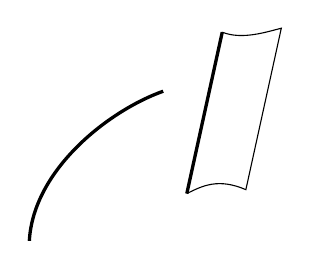
\begin{tikzpicture}[x=1cm,y=1cm]
\draw[very thick] (0,0) .. controls (.05,.9) and (1,1.65) .. (1.7,1.9);
\draw[very thick] (2,0.6)--(2.45,2.65);
\draw (2.45,2.65) .. controls (2.7,2.55) and (3,2.65) .. (3.2,2.7)--(2.75,.65) .. controls (2.4,.8) and (2.2,.7) .. (2,.6);
\end{tikzpicture}}

\diagram{\begin{tikzcd}[ampersand replacement=\&]
P_1^{+0}\subset A^1\arrow[r]\&A_2\supset P_2^+
\end{tikzcd}}
\deleted{$\unsure{D}+{}$}\quad $D'+nD\in P_2^+$
\[\begin{aligned}
(D'+nD)^3={}&D^{\unsure{\prime|!}3}+3nD'^2D\\
&+3n^2D'D^2+n^3D^3
\end{aligned}\]
\figure{\begin{tikzpicture}[x=1cm,y=1cm]
\draw (2.7,1.4) .. controls (3,1.6) and (3.3,1.7) .. (3.5,1.7);
\draw (0,0) .. controls (.05,.35) and (.4,.75) .. (.65,.9);
\draw (1.5,-.05) .. controls (1.9,.1) and (2,.3) .. (2.05,.5);
\draw[very thick] (3,.15) .. controls (3.35,.35) and (3.55,.6) .. (3.65,.9);
\node[draw,below] at (1.9,-.2) {$D^3\geq0$};
\end{tikzpicture}}
\figure{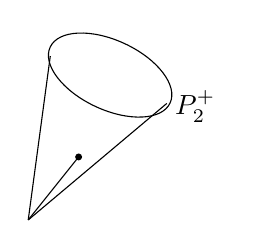
\begin{tikzpicture}[x=.8cm,y=.8cm]
\draw[rotate around={-25:(1.3,2.3)}] (1.3,2.3) ellipse (1.05 and .55);
\draw (0,0)--(.35,2.6) (0,0)--(2.2,1.85);
\draw (0,0)--(.8,1);\fill (.8,1) circle (.055);
\node at (2.65,1.8) {$P_2^+$};
\end{tikzpicture}}
\deleted{$\unsure{D+\frac1n D'}$}
\[D'+nD\simeq\]
\margin{99}
